\documentclass[twoside]{article}


\usepackage[sc]{mathpazo} % Use the Palatino font
\usepackage[T1]{fontenc} % Use 8-bit encoding that has 256 glyphs
\linespread{1.3} % Line spacing - Palatino needs more space between lines
\usepackage{microtype} % Slightly tweak font spacing for aesthetics

\usepackage[hmarginratio=1:1,top=32mm,columnsep=20pt]{geometry} % Document margins
\usepackage{multicol} % Used for the two-column layout of the document
\usepackage[hang, small,labelfont=bf,up,textfont=it,up]{caption} % Custom captions under/above floats in tables or figures
\usepackage{booktabs} % Horizontal rules in tables
\usepackage{float} % Required for tables and figures in the multi-column environment - they need to be placed in specific locations with the [H] (e.g. \begin{table}[H])
\usepackage{hyperref} % For hyperlinks in the PDF

\usepackage{lettrine} % The lettrine is the first enlarged letter at the beginning of the text
\usepackage{paralist} % Used for the compactitem environment which makes bullet points with less space between them

\usepackage{titlesec} % Allows customization of titles
\renewcommand\thesection{\Roman{section}} % Roman numerals for the sections
\renewcommand\thesubsection{\Roman{subsection}} % Roman numerals for subsections
\titleformat{\section}[block]{\large\scshape\centering}{\thesection.}{1em}{} % Change the look of the section titles
\titleformat{\subsection}[block]{\large}{\thesubsection.}{1em}{} % Change the look of the section titles

\usepackage{fancyhdr} % Headers and footers
\pagestyle{fancy} % All pages have headers and footers
\fancyhead{} % Blank out the default header
\fancyfoot{} % Blank out the default footer
\fancyhead[C]{Audio to MIDI} % Custom header text
\fancyfoot[RO,LE]{\thepage} % Custom footer text


\usepackage{multicol}
\usepackage{multirow}
% \setlength{\columnseprule}{0.4pt}
\usepackage{listings}
\usepackage{graphicx}
\usepackage{caption}
\usepackage{subcaption}
\usepackage{hyperref}
\usepackage{color}
\usepackage{float}
\usepackage{mathtools}
\usepackage{amssymb}
\usepackage{wrapfig}
\usepackage{amsmath}
\newcommand{\RN}[1]{%
  \textup{\uppercase\expandafter{\romannumeral#1}}%
}
\lstset{ %
language=Matlab,                % choose the language of the code
basicstyle=\footnotesize,       % the size of the fonts that are used for the code
numbers=left,                   % where to put the line-numbers
numberstyle=\footnotesize,      % the size of the fonts that are used for the line-numbers
stepnumber=1,                   % the step between two line-numbers. If it is 1 each line will be numbered
numbersep=5pt,                  % how far the line-numbers are from the code
backgroundcolor=\color{white},  % choose the background color. You must add \usepackage{color}
showspaces=false,               % show spaces adding particular underscores
showstringspaces=false,         % underline spaces within strings
showtabs=false,                 % show tabs within strings adding particular underscores
frame=single,           % adds a frame around the code
tabsize=2,          % sets default tabsize to 2 spaces
captionpos=b,           % sets the caption-position to bottom
breaklines=true,        % sets automatic line breaking
breakatwhitespace=false,    % sets if automatic breaks should only happen at whitespace
escapeinside={\%*}{*)}          % if you want to add a comment within your code
}
%----------------------------------------------------------------------------------------
%	TITLE SECTION
%----------------------------------------------------------------------------------------

\title{\vspace{-15mm}\fontsize{24pt}{10pt}\selectfont\textbf{Summary of Audio to MIDI }} % Article title

\author{
\large
\textsc{Li Yicheng}\thanks{\href{https://github.com/IAMLYCHEE?tab=repositories}{github link: https://github.com/IAMLYCHEE} }\\[2mm] % Your name
\normalsize t-yicli @ microsoft.com\\
\normalsize email: l.y.c.liyicheng@gmail.com \\ % Your institution
\normalsize Microsoft Xiao ICE \\
\vspace{-5mm}
}

\date{}
%----------------------------------------------------------------------------------------

\begin{document}

\maketitle

% \begin{multicols*}{2}
\section{Step 1, read and seperate an audio file}
\subsection{Read}
We use the librosa to help us read a .wav file , we need to specify the sampling rate and whether the source is sterero or monotone.\\

\textbf{sample code}
\begin{lstlisting}
audio_file = 'filename.wav'
audio, sr = librosa.load(audio_file, sr=48000, mono=True)
\end{lstlisting}
The audio is an array of size (duration of the music(in seconds) $\times$ 48000).
\subsection{Seperate}
Then we need to seperate a piece of music into several pieces. A music data can be very long with respect to the time and the sampling rate. A 48k music, which sample 48000 samples at each second, would generate 480000 data if it is 10s long. \\
Three terms are introduced:\\
\textbf{hop length}: hop length means how much a sliding window moved every time.\\
\textbf{window length}: window length for a frame of music, if too short, features are not easily 
to be found, however, if too long, unuseful information would sabotage one frame of music.\\
\textbf{frame}: a frame, is the cropped music data piece with the desinated window size.\\

\begin{figure}[H]
   \centering
   \includegraphics[width = 0.75\textwidth]{seperate.png}  
   \caption{divide a music piece}
\end{figure}
\textbf{sample code}
\begin{lstlisting}
# frame_amount is how many frames will we get
# this block is to seperate the seqs
hop = 128
frameSize = 1024
# now create a space to store the seqs
seqs = np.zeros((frame_amount, frameSize))
# Now we put the blocks into the seqs
for i in np.arange(0, len(audio) - frameSize, hop):
    seqs[i // 128, :] = audio[i:i + frameSize]
\end{lstlisting}
In my model, I used the hop size to be 128 and the frameSize to be 1024, and sample rate(sr) to be 48000.So if I have a song with length $l$ ( in seconds), I would have $frame\_amount = (l\times 48000 - 1024)/128$, so $ frame\_amount = (l \times sr - frame\_size)/hop\_size$ \\
\subsection{Parameters in this step}
\textbf{hop\_size},     \textbf{frame\_size},    \textbf{sample\_rate}

\section{Step2: STFT and Salient function}
\subsection{STFT}
\textbf{Mathematical}\\
$ \mathbf {STFT} \{x[n]\}(m,\omega )\equiv X(m,\omega )=\sum _{n=-\infty }^{\infty }x[n]w[n-m]e^{-j\omega n}$\\
\textbf{How to perform here}\\
For each frame, FFT is performed, since we are dealing with discrete data and we need to avoid Gibbs phenominent, a window is added before performing the FFT. Details of the reason is omitted here, and I the window shape I choose is the $hanning$ window. \\
Then is to choose the size of the FFT kernel, here I choose $n\_FFT=8192$, that means the resolution of our frequency axis is $\frac{sr}{n\_fft} = \frac{48000}{8192} = 5.86H_Z$\\
The FFT together with the seperate part above is called the STFT, and we can directly call the function in librosa to help use get the result of FFT of each frame, after the STFT we perform the normalization :$X(k)$ is the spectrum we get, $W(n)$ is the window sequence we choose.  $X_{normal} = \frac{2|X(k)|}{\displaystyle \sum_{0}^{l_f - 1} W_{hann}(n)}$\\
\textbf{sample code}
\begin{lstlisting}
win_length = 1024
window = 'hann'
n_fft = 8192
hop_length = 128
X = librosa.stft(audio, n_fft=n_fft, hop_length=hop_length,
                 win_length=win_length, window=window)
X_Normal = 2 * np.absolute(X) / np.sum(np.hanning(win_length))
\end{lstlisting}
% \end{multicols*}
\textbf{output dimension:}\\
if you can calculate the dimension with out look at below deduciton, you know STFT\\
else check the below:\\
if we have a music piece of 10s , then we would have a length $10\times sr = 10 \times 48000 = 480000$ vector.\\
Then we seperate it with  $hop\_size(l_h) = 128 $ and $frame\_size(l_f) = 1024$. We would get $(l_{vector} - l_f )/l_h = (480000-1024)/128 = 3742$ frames\\
each frame we perform a FFT of size $n_{fft} = 8192$, So we would get a vector with length 8192 for each frame. \\
To conclude, we would get a two-dimension array with size $frame_{amount} \times n_{fft} = 3742 \times 8192$

\begin{figure}[H]
    \centering
    \begin{subfigure}[b]{0.45\textwidth}
        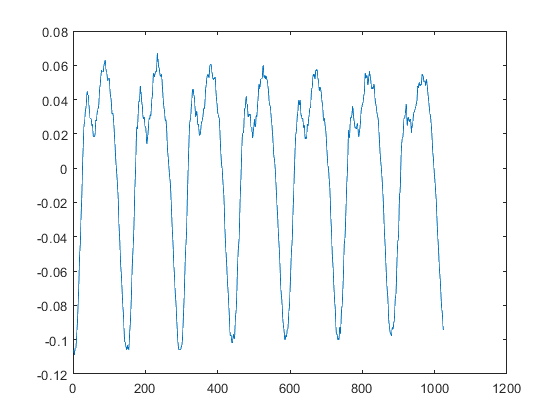
\includegraphics[width=\textwidth]{oneFrame.png}
        \caption{one frame of audio data}
    \end{subfigure}
    ~ %add desired spacing between images, e. g. ~, \quad, \qquad, \hfill etc. 
      %(or a blank line to force the subfigure onto a new line)
    \begin{subfigure}[b]{0.45\textwidth}
        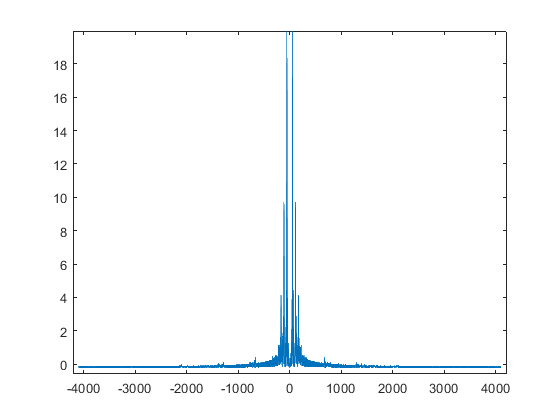
\includegraphics[width=\textwidth]{specOneFrame}
        \caption{the spectrum of that frame}
    \end{subfigure}
    \caption{Example DFT}
\end{figure}
\noindent From the figure, I showed that a frame with size$1024$, generate a spectrum vector with size$8192$.

\subsection{Crop data}
Obviously the data with size $frame_{amount} \times n_{fft}$ is very large and most of the frequency in the spectrum is not need for this job, So the data is cropped.\\
The minimum and maximum frequency I choose for this model is 55 Hz and 1760 Hz. Now I find the corresponding index in the spectral and crop the 2-dimension array.\\
\begin{lstlisting}
# Crop the data to increase the speed
freq_min = 55
freq_max = 1760
k_min = np.floor(freq_min * n_fft / sr)
k_max = np.floor(freq_max * n_fft / sr)
X_Crop = X_Normal[int(k_min): int(k_max), :]
\end{lstlisting}
The resolution of the spectral is $resolution =\frac{sr}{n_fft} = 5.86 $, therefore, after the cropping, for each frame we would have  a length of $spec_{amount} = (freq_{max} - freq_{min} )/ resolution = (1760-55)/5.86=290$ vector.
So after this step, for a 10s audio, we have $frame_{amount} \times spec_{amount} = 3742\times 290$ array data.\\

\subsection{Salient Function}
The extracted spectral peaks are used to construct a salience function, a representation of pitch salience over time. The peaks of this function form the F0 candidates for the main melody. The salient function in my model is based on harmonic summation. \\
For the spectral of each frame, the top 5 peaks are chosen and the location of each is assigned with the weight to find the $F_0$ frequency of the melody. This is done by calling the salience function in librosa.\\
\textbf{Sample Code}\\
\begin{lstlisting}
# now we perform the salience function
freqs = np.linspace(freq_min, freq_max, num=X_Crop.shape[0])
harms = [1, 2, 3, 4, 5]
weights = [1.0, 0.45, 0.33, 0.25, 0.10]
S_sal = librosa.salience(X_Crop, freqs, harms, weights, fill_value=0)
\end{lstlisting}
\fbox{
  \parbox{\textwidth}{
  	!!!!!This part is removed from model 1.0 to model 2.0, since the cropped spectral already provides us with each information
  }
}

\subsubsection{gather information of top 3 peak location in the spectral}
\textbf{Sample Code}
\begin{lstlisting}
    iFrame = X_Crop[:, i]
    peakInd = detect_peaks(iFrame)
    local_max_Peaks = iFrame[peakInd]
    # sort the amplitudes and find the stornges ones using sort
    indSort = np.argsort(local_max_Peaks)
    # find the frequency according to the index
    sortedLocs = peakInd[indSort]
    sortedLocs = sortedLocs[::-1]
    # put them into the memery space
    # just the first three strongest
    if sortedLocs.shape[0] >= 3:
        pks_locs[i, :] = sortedLocs[0:3]
    else:
        pks_locs[i, :] = np.array([0, 0, 0])
\end{lstlisting}


\section{Step3: Other features}
Calculate other information from the audio data $x[n]$.
\subsection{Energy}
Calculate the energy of each frame :$E = log (\displaystyle \sum_{0}^{l_f - 1} x[n]^2)$\\ 
\textbf{Sample Code}
\begin{lstlisting}
E = np.multiply(seqs, seqs)
E = np.sum(E, axis=1)
E[np.where(E < 0.0000001)] = 0.00001
E = np.log10(E)
\end{lstlisting}

\subsection{zero crossing}
Calculate how many times it cross a zero:$Z_c = \displaystyle \sum_{1}^{l_f} (|sgn(x[n]) - sgn(x[n-1])| == 2)$\\
\textbf{Sample Code}
\begin{lstlisting}
    indexs = np.diff(np.sign(seq))
    indexs = np.abs(indexs)
    zeros_pos = np.array((np.where(indexs == 2)))
    zeros_cros[i] = zeros_pos.shape[1]
\end{lstlisting}


\subsection{Auto-correlation}

Also use the auto-correlation to find whether a signal has some feature perform likes a noise : $R_x =  \frac{\displaystyle \sum_{n=1}^{l_f} x[n][n-1]}{\sqrt{(\displaystyle \sum_{n=1}^{l_f-1}x[n]^2)(\displaystyle \sum_{n=1}^{l_f-1}x[n-1]^2)}}$\\

\textbf{Sample Code}
\begin{lstlisting}
    numerator = np.sum(np.multiply(seq[1:frameSize], seq[0:frameSize - 1]))
    denominator = np.sqrt(np.sum(np.multiply(seq[1:frameSize], seq[1:frameSize])) *
                          np.sum(np.multiply(seq[0:frameSize - 1], seq[0:frameSize - 1])))
    if denominator == 0:
        denominator = 0.0001
    auto_corr[i] = numerator / denominator
\end{lstlisting}

\section{Step4:Self-clustering and First Cut}
\subsection{form the dataset}
now we gather all the feature data of all frame: That is we form a dataset with dimension$frame_{amount} \times 5$, the five features are: [energy, zero crossing amount, autocorrelation, top two peaks location].\\
After concatenate all the feature vectors , we normalize the data since we would use kmeans clustering in the next step.\\
\textbf{Sample Code}
\begin{lstlisting}
# concatenate along the features
dataSet = np.concatenate((E, zeros_cros, auto_corr, pks_locs[:, 0:2]), axis=1)
# now perform the zscore, because we would use kmeans to cluster
from scipy import stats
dataSet = stats.zscore(dataSet, axis=0)
\end{lstlisting}

\subsection{clustering with predefined centroid}
After several experiments, I found out that: \\
$\bullet 1:$ The vocal part has more energy\\
$\bullet 2:$ The vocal part with the pitch we want has the smallest frequency\\
$\bullet 3:$ The vocal part has the most autocorrelation\\
$\bullet 4:$ The vocal part with the pitch we want has the pitch just greater than the silence\\
Therefore, the initial centroid I chose is :
$\begin{bmatrix}
1 & -1 & 3 & 0 & 0 \\
0 & 0 & 2 & -1 & -1 \\
-2 & 2 & 1 & 2 & 1 \\
-3 & 3 & 0 & 3 & 3 \\
\end{bmatrix}
$\\
Class 0 is the frames that most probably contains the audio information, the other three classes contains information of breath, silence and noise. Then we can mark the boundaries from non-audio to audio, using the derivative of the labels.The following figure show the example of audio file 'vocal\_xiaobin'\\
\textbf{Sample Code}\\
\begin{lstlisting}
start_matrix = np.array([[1, -1, 0, 0, 0],
                         [0, 0, 1, -1, -1],
                         [-2, 2, 2, 2, 1],
                         [-3, 3, 3, 3, 3]])
# clustering
kmeans = KMeans(n_clusters=4, init=start_matrix,n_init = 1).fit(dataSet)
# generate the labels
pyidx = kmeans.labels_
# let the label above 1 to be 1, the expected sound place is labeled zero
pyidx[np.where(pyidx>0)] = 1
#differentiate the label
diff_pyidx = np.diff(pyidx)
\end{lstlisting}

\begin{figure}[H]
   \centering
   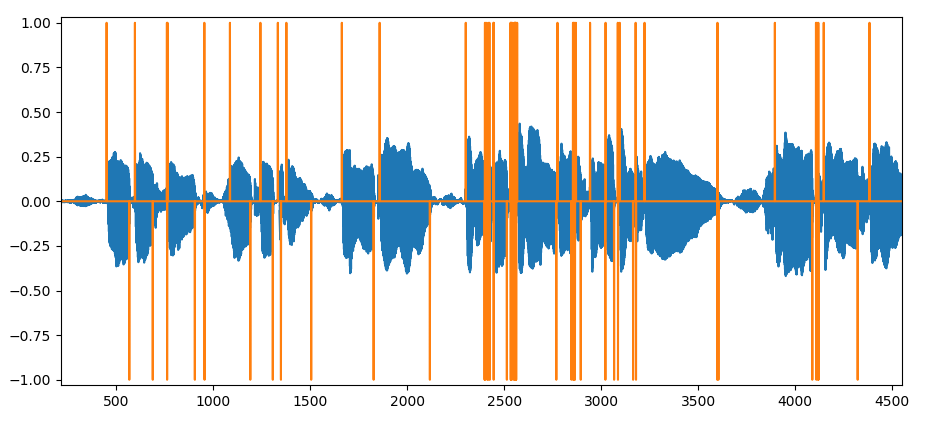
\includegraphics[width = 0.8\textwidth]{first_cut.PNG}  
   \caption{Cut with cluster label, 1 means on and -1 means off}
\end{figure}


\section{Step 5:Optimizing on audio Cut}
There are some problems of the step 4, first, some places may need to be cut(show in red arrow) and some place should not be cut(show in blue arrow)\\
\begin{figure}[H]
   \centering
   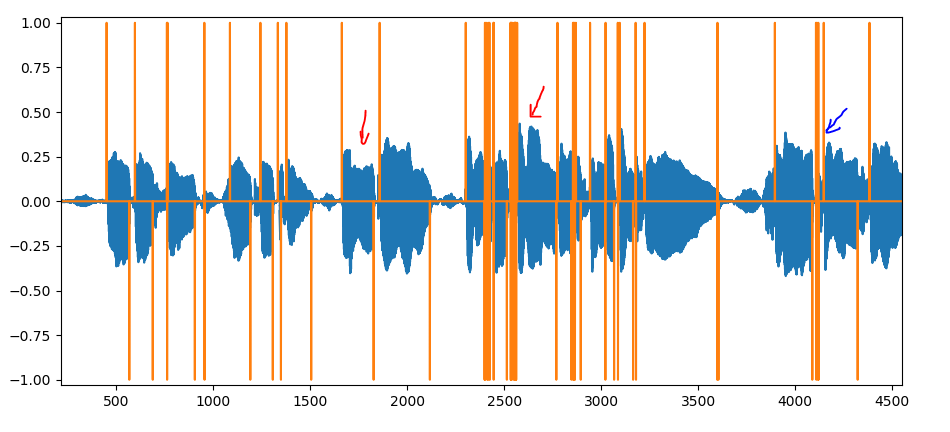
\includegraphics[width = 0.8\textwidth]{first_cut_mark.PNG}  
   \caption{Some wrong places}
\end{figure}

\subsection{Optimize Algorithm}
$\bullet 1$ after first cut, we get several \textbf{blocks} with durations, for \textbf{duration < 15 frames}, we delete that cut.\\
$\bullet 2$ For \textbf{duration > 215 frames}, we perform the find break operation.\\
\textbf{Details in find break:}\\
I use the energy information to find more breaks, first for each block we find the corresponding energy. The right is the energy and the red circle marks the block we need to deal with.\\
\begin{figure}[H]
   \centering
   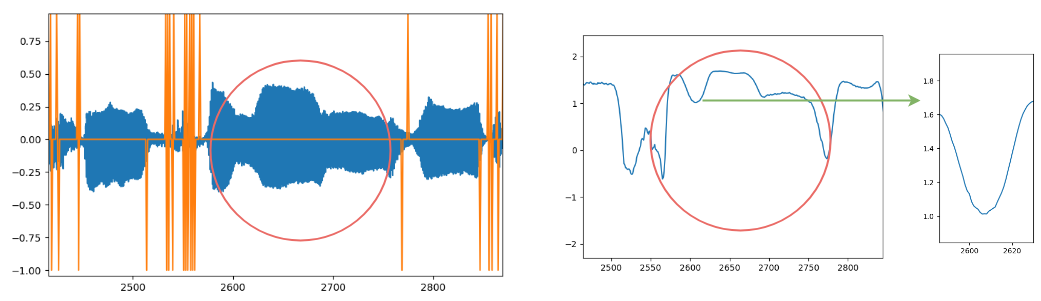
\includegraphics[width = 0.95\textwidth]{findbreak.png}
   \caption{find the concave}
\end{figure}
I set some threshold to mark whether the concave indicates a break or not. The concave detect and break determination is explained below:\\
\textbf{Algorithm}
\begin{lstlisting}
determine a sliding window, and hop size for the block
the first half of the sliding window, calculate the sum of the derivative and times -1
the next half of the sliding window, calculate the sum of the derivative 
add two sums together and set a threshold to see whether that window contains a concave
find the position contains concave, find the area of the concave, because I found out that some peaks are small but continous,menas there is a slowing concave. Some are high but narrow which means a sharp concave. So use area to determine. The are I chose is 6.0.
find the final location of the concave
 \end{lstlisting} 
 \textbf{sample code}\\
too long, put in the appendix\\
$\bullet 3$ delete the small blocks again.
\begin{figure}[H]
   \centering
   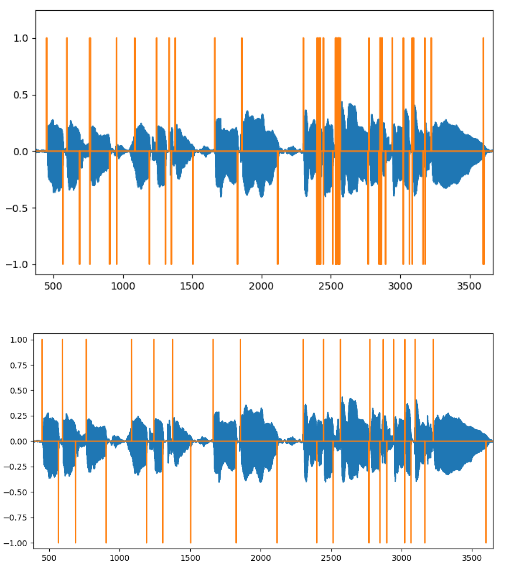
\includegraphics[width = 0.75\textwidth]{optimize.png}  
   \caption{effect of cutting optimization,top: first cut, below: Optimization}
\end{figure}

\section{Step 6: Pitch Selection For MIDI}
\subsection{Summary}
This part, we need to find the pitch line for each block. The data we use is the peak location we get at the beginning. After the STFT, we find the top 3 peaks and their corresponding locations and choose the smallest location as the pitch of that frame.\\
\textbf{Algorithm}\\
\begin{lstlisting}
perform stft for each block, find the smallest location which has the top3 frequency response
transform from location to pitch value
delete the pitch outlier data with the neighbour block pitch information
use the median filter with size S and mode 'reflect'
round the result
further smooth with some rules
\end{lstlisting}

\begin{figure}[H]
   \centering
   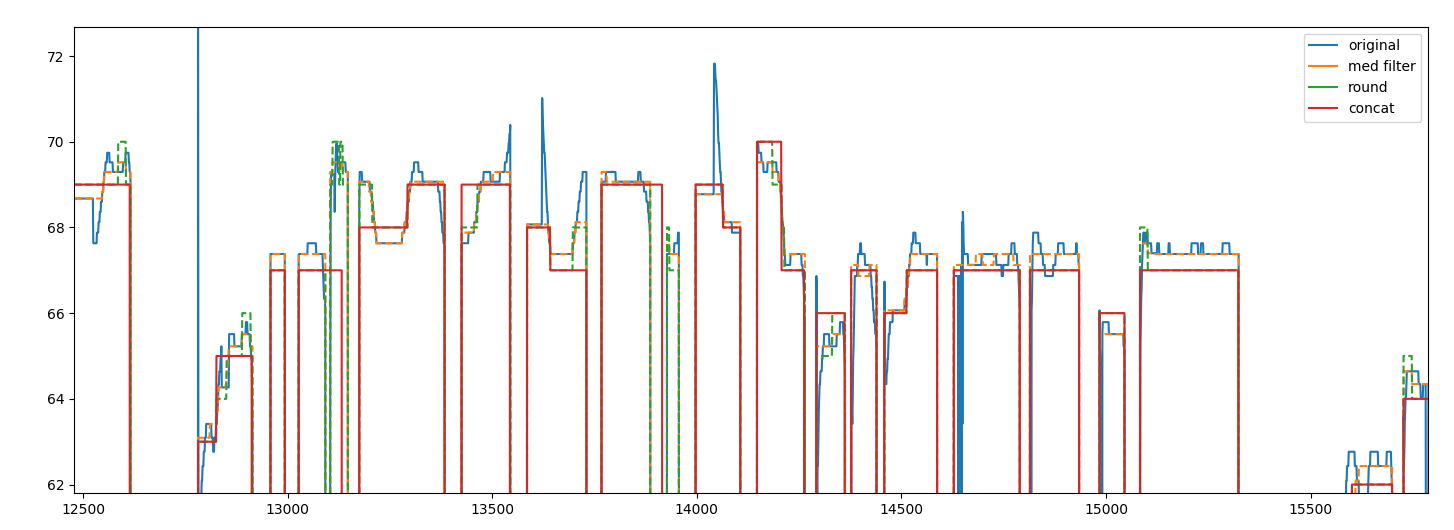
\includegraphics[width = 0.95\textwidth]{pitch_selection.png}  
   \caption{Summary of find the pitch line}
\end{figure}

\subsubsection{step 1}
From the last part, we already get the pitch on and pitch off information. And I call each audio piece in one pitch-on and pitch-off pair a block. Perform the stft in each block, with hop size 128 and window length 1024. Then we crop the spectrum to limit the frequency response in 55 Hz to 1760 Hz. Find the top 3 strongest peaks in spectrum. Choose the smallest location.\\

\begin{figure}[H]
    \centering
    \begin{subfigure}[b]{0.45\textwidth}
        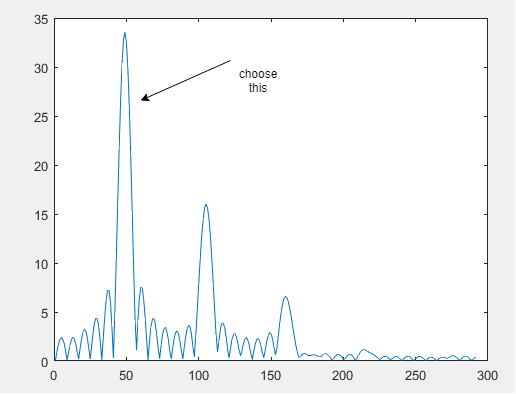
\includegraphics[width=\textwidth]{freqchoose.png}
        \caption{example}
    \end{subfigure}
    ~ %add desired spacing between images, e. g. ~, \quad, \qquad, \hfill etc. 
      %(or a blank line to force the subfigure onto a new line)
    \begin{subfigure}[b]{0.45\textwidth}
        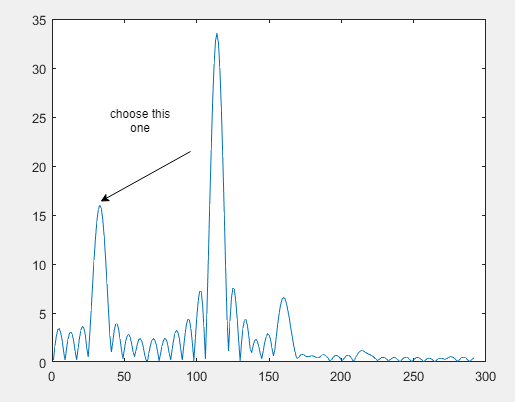
\includegraphics[width=\textwidth]{freqchoose2.png}
        \caption{example}
    \end{subfigure}
    \caption{choose the smallest location}
\end{figure}

\subsubsection{transform to pitch value}
$freq_{hz} = 55 + (1760 - 55) / 291 * location$\\
$pitch_{midi} = 12 * np.log2(32 * freq_{hz} / 440) + 9$\\

\noindent After this step we get the response shown in blue color in figure 7. 

\subsubsection{delete the outlier}
\textbf{1.}Gather all the pitches in the current block and the previous block and the next block. \\
\textbf{2.}Calculate the pitches mean $\mu_p$\\
\textbf{3.}Calculate the pitches standard deviation $\sigma_p$\\
\textbf{4.}Find the pitch that i $> \mu_p + 1.5 * \sigma_P$\\
\textbf{5.}change the pitch of that location as the mean of the rest pitches.\\

\noindent After this step some extremely strange pitch that suddenly errupts would be deceased.\\

\subsubsection{smooth the pitches}
I performed a median filter with size 93 (0.25s) to smooth the pitch data. The rsult is shown in the orange line in figure 7\\

\subsubsection{round the pitches}
Then is to round the float number to the nearest integer pitch.

\subsection{final Optimization}
\begin{multicols}{2}
\begin{figure}[H]
   \centering
   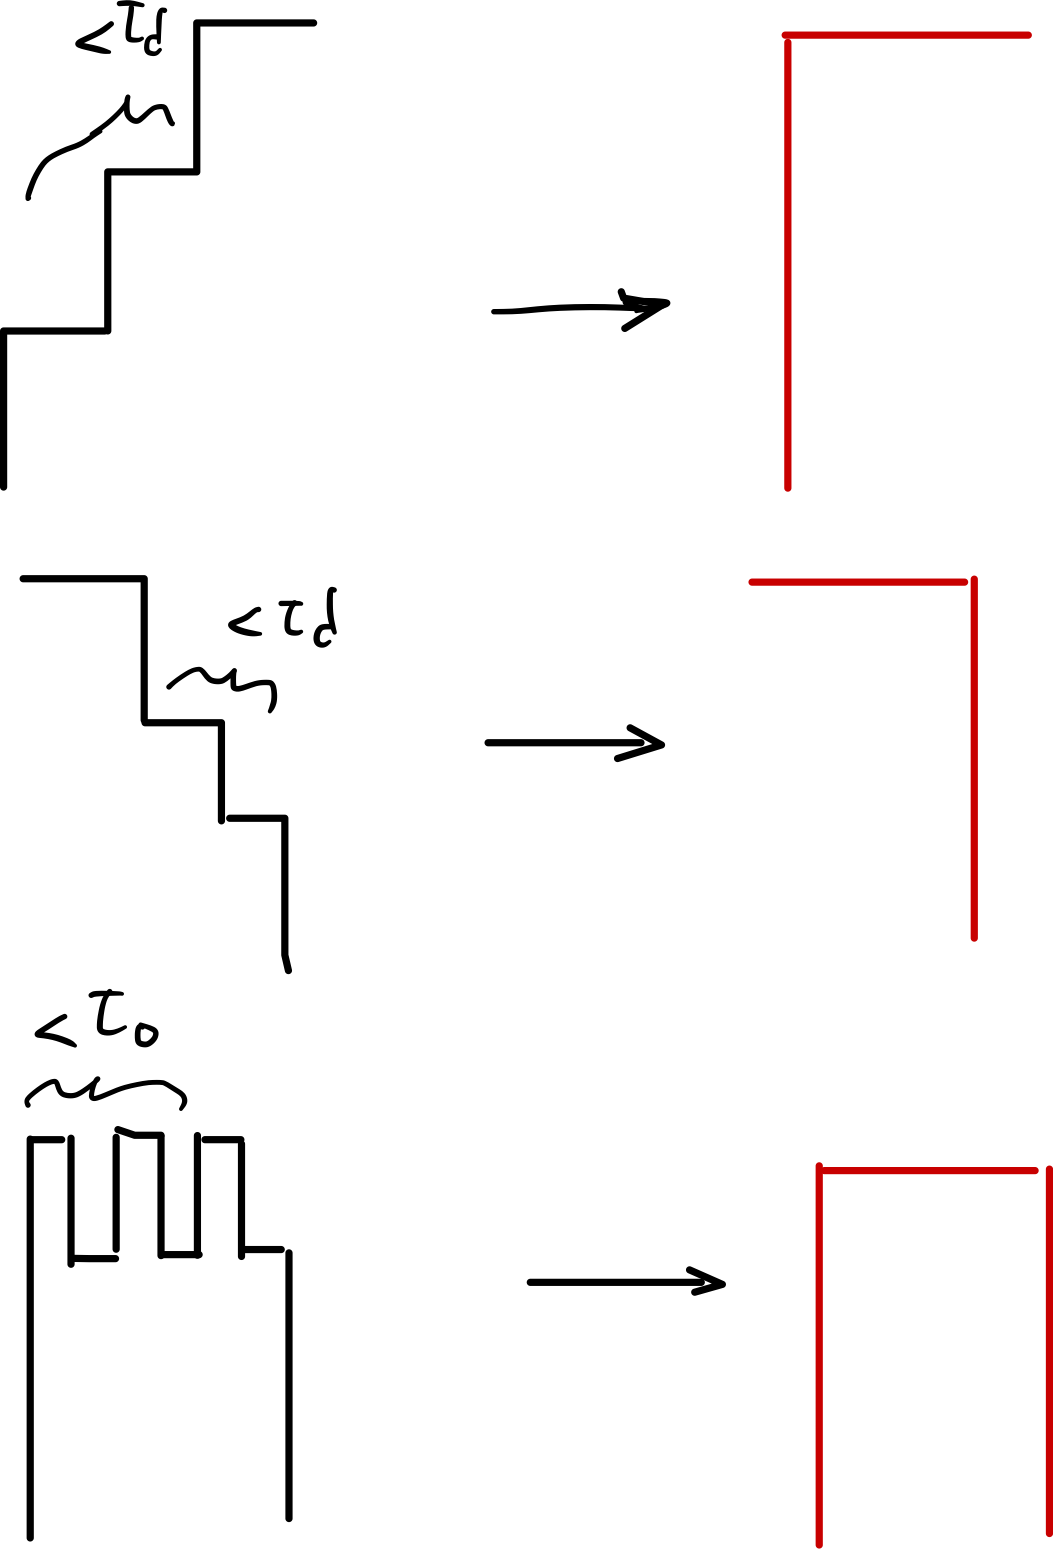
\includegraphics[width = 0.4\textwidth]{final_op.png}  
   \caption{final optimization}
\end{figure}
This is to increase the continuity of the midi format, if we stop above , the pitches would be changing very soon and we would get a lot of pitches in each block. This step we suppress the sharp rising and sharp decreasing and small oscillation. I made sure each pitch would last more than 0.1 second and caoncatenate blocks with the same pitch and close to each other.  When a sound raises, it generally starts from a low frequency to a desired frequency, most of the time the rising is very fast, if we let this rising exist, when transform to midi, new note with very small duration would be added and the effect is not good, that is not the melody we would like to extract, so the duration is accumulated until meet some requirement. And the pitch when the requirment met is set to the pitch we want.
\end{multicols}
\end{document}